%% Paper 2 -- Version Migration as a Correlated Shock (IEEE-Access-style draft).
%% Self-contained two-column article (compiles with base pdflatex). For the official
%% IEEE Access submission, port this text into the ieeeaccess.cls template on Overleaf.
%% Numbers are the frozen two-pair credit-task analysis (openai_nano, gemini_flash).
\documentclass[10pt,twocolumn]{article}
\usepackage[letterpaper,margin=0.72in,columnsep=0.28in]{geometry}
\usepackage{amsmath,amssymb}
\usepackage{booktabs}
\usepackage{graphicx}
\graphicspath{{figures/}}
\usepackage{times}
\usepackage[colorlinks=true,urlcolor=blue,citecolor=blue,linkcolor=black]{hyperref}
\setlength{\parskip}{2pt}
\renewcommand{\baselinestretch}{1.02}

\begin{document}
\twocolumn[{%
\centering
{\LARGE\bfseries Version Migration as a Correlated Shock:\\[3pt]
Model Updates as an Unmanaged Risk Channel in LLM-Based Financial Systems\par}
\vspace{0.9em}
{\normalsize First A. Author, \quad Second B. Author\par}
{\small [Department, Institution, City, Country]\quad \{first.author, second.author\}@domain.edu\par}
\vspace{1.0em}
\parbox{0.93\textwidth}{%
\small\textbf{Abstract---}Financial institutions deploying large language model (LLM) agents inherit a risk absent from classical model governance: when the vendor updates the model, every institution's agents shift behavior simultaneously and involuntarily. We run an identical, deterministic decision pipeline across two real vendor version migrations on a credit-health classification task---SAFE / WATCH / DISTRESS judged from each company's most recently reported quarterly financials, over 100 companies $\times$ 12 as-of dates $\times$ 3 replicates per version (3{,}600 calls per version, 7{,}200 per pair; 14{,}400 across both migrations)---and quantify the decision discontinuity induced purely by the update, separated from within-version sampling noise by a fixed per-cell seed. The ground truth is an objective, reproducible formula (Altman $Z''$ bands), and the models are competent (accuracy well above the three-way chance rate), so the effect is not an artifact of a task no model can perform. We report three findings. \emph{First}, both migrations produce a large, highly significant shock: the OpenAI update (\texttt{gpt-5-nano-2025-08-07}$\to$\texttt{gpt-5.4-nano}) flips 0.112 of assessments above the noise floor (95\% CI [0.077, 0.150]) and the Gemini update (\texttt{gemini-2.5-flash}$\to$\texttt{gemini-3.5-flash}) flips 0.381 (95\% CI [0.303, 0.458]). \emph{Second}, a prevalence/churn decomposition shows the two shocks are structurally \emph{opposite}: OpenAI's is genuine per-company reconsideration biased toward DISTRESS (churn 0.122 $>$ marginal shift 0.095), while Gemini's is a wholesale distributional shift toward SAFE (marginal 0.319 $\gg$ churn 0.070) that moves 0.201 of the book's credit tiers. \emph{Third}, neither update improves accuracy against ground truth, so the shock is forced turnover without compensating skill. That two vendor updates perturb the identical task in opposite directions by different mechanisms shows migration risk is idiosyncratic and unpredictable across vendors---a synchronized, un-hedgeable channel that model-risk guidance does not contemplate; indeed, the 2026 revised guidance (SR 26-2, which superseded SR 11-7) places generative AI outside its scope entirely. We propose pre-migration parallel-run monitoring metrics to detect it and release a frozen, deterministic artifact that reproduces every number.

\vspace{0.55em}
\noindent\textbf{Index Terms---}large language models, model risk management, SR 11-7, algorithmic monoculture, model updates, model drift, computational finance, credit risk, reproducibility, pre-registration.}
\vspace{1.4em}
}]

\section{Introduction}
Large language models are increasingly embedded in financial decision pipelines---credit and counterparty screening, disclosure and filing review, alerting and triage---where a model's output feeds a downstream action. Classical model-risk management assumes the institution controls its models: a model is developed, validated, and changed on the institution's own schedule, and a change triggers revalidation~\cite{sr117}. Foundation-model deployment breaks that assumption. The model is a third-party service that the vendor updates on its own schedule and frequently deprecates, so continued operation forces migration. The result is a risk with no analog in the pre-foundation-model era: at the moment of a vendor update, the behavior of \emph{every} institution running that model shifts at once, involuntarily, and---because they share the model---in a correlated way.

Whether this shift is large or negligible is not a foregone conclusion; it is the subject of two competing intuitions. The \emph{continuity} view holds that a point release is a modest refinement, that vendors preserve behavior for backward compatibility, and that a fixed, deterministic pipeline should therefore see few decisions change. The opposing \emph{discontinuity} view holds that a version is a fresh training run with different data, objectives, and alignment, so held-fixed inputs can produce materially different decisions. These predictions are far apart---from an excess flip rate near zero (migration is benign) to a large one (migration silently rewrites decisions)---so measuring it is a genuine test, not a restatement of intuition. We resolve it empirically for two real, vendor-declared ``recommended replacement'' migrations, and find not only that the effect is large for both, but that its \emph{direction and mechanism differ across vendors}, which is itself the sharpest governance implication.

Despite the ubiquity of vendor updates, the quantity that governs their operational risk---how much a migration changes graded decisions, and \emph{how}---is rarely measured with statistical rigor. Two obstacles recur. (i) \emph{Noise confound}: a model re-invoked on the same input does not answer identically, so raw before/after disagreement conflates migration with sampling variance. (ii) \emph{Mechanism ambiguity}: a change in the mix of labels (the whole book re-rated) is very different, operationally, from a change in \emph{which} names are re-judged, yet a single flip-rate number cannot tell them apart. Our contribution is to measure the magnitude \emph{net of} the noise floor and to decompose it into a marginal (prevalence) component and a genuine per-name churn component---neither of which follows from the intuition that ``updates change things.''

\noindent\textbf{Contributions.} (1) A pre-registered, reproducible measurement of version-migration decision instability on a real, objectively-graded financial task, with an explicit within-version noise floor, over two vendor migrations. (2) A prevalence/churn decomposition, with three chance-corrected agreement statistics, that reveals the two migrations are structurally opposite rather than merely different in size. (3) An outcome linkage against an objective ground truth (Altman $Z''$) establishing that the shock buys no reliable accuracy in either case. (4) A mapping to the SR 11-7 provisions that presuppose institution-controlled model change, and a proposed pre-migration parallel-run monitoring metric. (5) A released, deterministic artifact (frozen data, seeded analysis, build-gated numbers) that reproduces every figure and table.

\section{Related Work}
\subsection{Model-update regression in general ML}
A model update silently overturning previously-correct predictions is documented outside finance. MUSCLE~\cite{muscle} names these ``negative flips'' across LLM updates and proposes a compatibility adapter to reduce them; the reliable-change literature formalizes when an instance-level change exceeds within-model noise~\cite{reliable}; and update-governance work studies testing regimes for the LLM supply chain~\cite{supply}. Underspecification analyses further show that held-fixed prompts leave much to the model, so updates can regress silently on requirements never stated~\cite{underspec}. Our contribution is orthogonal on three axes: we measure the effect as a \emph{correlated, cross-institution} risk rather than a per-model engineering defect; we situate it in a \emph{financial decision} task with an objective, consequential ground truth; and we tie it to \emph{model-risk governance}.

\subsection{Algorithmic monoculture and systemic risk in finance}
A parallel literature argues that convergence on shared foundation models creates correlated failure and systemic fragility in markets~\cite{kim,systemic,homog}, and supervisory bodies have begun to flag AI homogenization as a systemic concern~\cite{esrb}. That work is largely conceptual or market-microstructure theory, reasoning about correlated \emph{trading} behavior at the market level. We provide the missing empirical, decision-level complement: a controlled measurement of how a single vendor update perturbs concrete, graded decisions, which is the mechanism by which such correlation would actually enter an institution's book.

\subsection{Agreement, prevalence, and the kappa paradox}
Chance-corrected agreement statistics---Cohen's $\kappa$, Scott's $\pi$, and Gwet's AC1~\cite{gwet}---are the standard tools for paired categorical agreement, and are known to diverge under skewed marginals (the ``$\kappa$ paradox''). We treat the two versions as paired raters and report all three, and we further separate the marginal shift from genuine reshuffling explicitly, so the mechanism is not left to the choice of statistic.

\subsection{Model risk management and generative AI}
SR 11-7~\cite{sr117} was the foundational US model-risk framework until it was superseded in April 2026 by the revised interagency guidance SR 26-2~\cite{sr2602}; SR 11-7 predates transformers and is silent on stochastic, vendor-updated models, and SR 26-2 explicitly places generative and agentic AI outside its scope. An emerging strand extends model-risk concepts to autonomous and agentic AI and proposes general validation and governance frameworks~\cite{mrm}. Our contribution is narrower and empirical: we make one specific, un-governed channel concrete and measurable---the synchronized shock of vendor version migration---and propose a monitoring metric to close it, rather than a general framework.

\subsection{Reproducibility and pre-registration}
Pre-registration and frozen, hash-verified datasets remain uncommon in empirical LLM studies. We adopt a confirmatory design---freeze the plan, collect once, re-analyze deterministically---and gate every reported number against the frozen analysis, releasing the artifacts.

\section{Problem Formulation and Metrics}
\subsection{Task and unit}
For a migration pair (an incumbent version $v_{\mathrm{old}}$ and its successor $v_{\mathrm{new}}$), the unit is a single-model credit-health classification per cell $s=(\text{company},\text{date},\text{replicate})$. The agent receives the company's most recently reported quarterly financials as of the date and emits a label $y \in \{\text{SAFE},\text{WATCH},\text{DISTRESS}\}$ in strict JSON with a conviction and rationale.

\subsection{Flip rate and the within-version noise floor}
Because the same version re-invoked on the same cell need not answer identically, we define a within-version noise floor: the fraction of within-version replicate pairs (same cell, different seed) whose label differs, pooled over both versions. The cross-version flip rate is the fraction of matched cells whose label differs between $v_{\mathrm{old}}$ and $v_{\mathrm{new}}$. The pre-registered \emph{primary endpoint} is
\begin{equation}
\text{excess flip} = \text{cross-version flip} - \text{within-version flip}.
\end{equation}

\subsection{Prevalence/churn decomposition}
Let $p_o(y),p_n(y)$ be the label shares under the two versions. The \emph{marginal shift} $\tfrac12\sum_y |p_n(y)-p_o(y)|$ is the minimum fraction of cells that must change to realize the new label mix (a wholesale re-rating). The \emph{churn} is the gross flip rate minus the marginal shift: genuine per-name reconsideration that cancels in aggregate. We also report Cohen's $\kappa$, Scott's $\pi$, and Gwet's AC1 between the paired labels. Directional drift is tested by a continuity-corrected McNemar test ($\mathrm{df}=1$) on the binary indicator of the most-severe tier (DISTRESS vs.\ not), which detects asymmetric movement into or out of distress; the full three-category generalization is Bowker's test on the $3\times3$ transition matrix, which we report as a consistency check.

\subsection{Version isolation and uncertainty}
A cell-parity seed, $\mathrm{SHA256}(\text{master}\,|\,\text{ticker}\,|\,\text{date}\,|\,\text{replicate})$, is identical for $v_{\mathrm{old}}$ and $v_{\mathrm{new}}$ at every cell, so the version is the only thing that differs (zero seed mismatches verified). Confidence intervals use a cluster bootstrap resampling companies (the clustering unit), 2{,}000 draws, fixed RNG seed 42, percentile method. A verdict of \textsc{Confirmed} requires excess flip $>0$ with a 95\% CI excluding zero.

\section{Experimental Design}
\subsection{Grid}
100 large-cap companies stratified across all 11 GICS sectors $\times$ 12 analysis dates in 2026 $\times$ 3 replicates $=$ 3{,}600 calls per version; with two versions this is 7{,}200 calls per migration pair, and 14{,}400 across the two pairs. Dates span distinct 2026 market regimes.

\subsection{No-lookahead documents}
For each cell the most recent quarterly filing with filing date strictly before the analysis date is selected and rendered as a human-readable summary (revenue, margins, income, assets, liabilities, working capital, retained earnings). Reported financials are immutable, so the document set is fetched once and frozen; the model never sees the ground-truth formula.

\subsection{Ground truth}
The objective label is the Altman $Z''$ band computed from the same statements: $Z''>2.6$ SAFE, $1.1$--$2.6$ WATCH, $<1.1$ DISTRESS. The $Z''$ model and these non-manufacturer / emerging-market cutoffs are the revised discriminant model of Altman~\cite{altman_em}, not the original 1968 $Z$-score~\cite{altman}, and are computed as $Z''=6.56X_1+3.26X_2+6.72X_3+1.05X_4$ from working capital, retained earnings, EBIT, and book equity over total assets/liabilities. Section~\ref{sec:disc} addresses the circularity objection this invites; briefly, the primary instability result never uses the label---only the secondary accuracy linkage does.

\subsection{Models and migrations}
Two vendor-declared ``recommended replacement'' migrations are studied (Table~\ref{tab:models}), each with a hard shutdown date that forces institutions to migrate. Decode temperature is 0; robustness across $T\in\{0,0.7,1.0\}$ is reported.

\begin{table}[t]
\centering
\caption{Migration pairs (exact snapshot strings pinned; hash-frozen data is the object of record).}
\label{tab:models}
\small
\begin{tabular}{@{}llc@{}}
\toprule
Pair & $v_{\mathrm{old}}\to v_{\mathrm{new}}$ & $v_{\mathrm{old}}$ shutdown \\
\midrule
openai\_nano & \texttt{gpt-5-nano-2025-08-07} $\to$ \texttt{gpt-5.4-nano} & 2026-12-11 \\
gemini\_flash & \texttt{gemini-2.5-flash} $\to$ \texttt{gemini-3.5-flash} & 2026-10-16 \\
\bottomrule
\end{tabular}
\end{table}

\subsection{Pre-registration, freezing, reproducibility}
The design (endpoints, grid, seeds, prompt, decision rule, Altman ground truth) was frozen and SHA-256-hashed \emph{before} any credit-task model call, so both pairs are confirmatory. Raw data are collected once into immutable, read-only, hash-stamped CSVs; the analysis reads only those plus the frozen configuration, with all randomness seeded, and a build gate rejects any reported number that disagrees with the frozen analysis.

\section{Results}
\subsection{Both migrations produce a large shock (primary)}
The primary endpoint is \textsc{Confirmed} for both pairs (Table~\ref{tab:main}). OpenAI's excess flip rate is 0.112 (95\% CI [0.077, 0.150]) over 3{,}490 matched cells---cross-version flip 0.217 against a within-version noise floor of 0.105---so the update overturns roughly one in nine credit assessments beyond what re-invoking the same model would produce. Gemini's is far larger, 0.381 (95\% CI [0.303, 0.458]) over 3{,}600 cells; because that incumbent is nearly deterministic across seeds (noise floor 0.008), almost the entire cross-version flip is excess.

\noindent\emph{Cell accounting.} Of 3{,}600 cells per version, OpenAI returned a valid label for 3{,}540 ($v_{\mathrm{old}}$) and 3{,}548 ($v_{\mathrm{new}}$); the matched-pair requirement---a cell is analyzed only if \emph{both} versions produced a valid label at the same seed---yields 3{,}490 analyzed cells. The $\sim$1.5\% per-version attrition is transient provider errors (HTTP 5xx) and a single JSON parse failure, distributed across sectors and dates, not a systematic drop on one arm. Gemini, after a daily-quota-limited backfill, returned 3{,}600/3{,}600 valid labels per version, so all 3{,}600 cells are matched.

\begin{table}[t]
\centering
\caption{Primary and secondary results for both migrations (OpenAI 3{,}490 matched cells; Gemini 3{,}600).}
\label{tab:main}
\small
\begin{tabular}{@{}lcc@{}}
\toprule
Quantity & OpenAI & Gemini \\
\midrule
Excess flip rate (primary) & 0.112 & 0.381 \\
\;\; 95\% CI & [.077,.150] & [.303,.458] \\
\;\; cross-version flip & 0.217 & 0.389 \\
\;\; within-version floor & 0.105 & 0.008 \\
Marginal (rating-mix) shift & 0.095 & 0.319 \\
Churn (genuine) & 0.122 & 0.070 \\
\;\; churn 95\% CI & [.083,.161] & [.029,.120] \\
Cohen $\kappa$ / Scott $\pi$ / Gwet & .60/.60/.70 & .33/.27/.47 \\
Credit-tier turnover & 0.108 & 0.201 \\
McNemar drift ($p$) & $6{\times}10^{-18}$ & $1.4{\times}10^{-59}$ \\
Drift direction & DISTRESS & SAFE \\
Accuracy old/new (chance .33) & .54/.56 & .49/.43 \\
Flip-cond.\ accuracy $\Delta$ & $+0.124$ & $-0.179$ \\
\bottomrule
\end{tabular}
\end{table}

\begin{figure}[t]
\centering
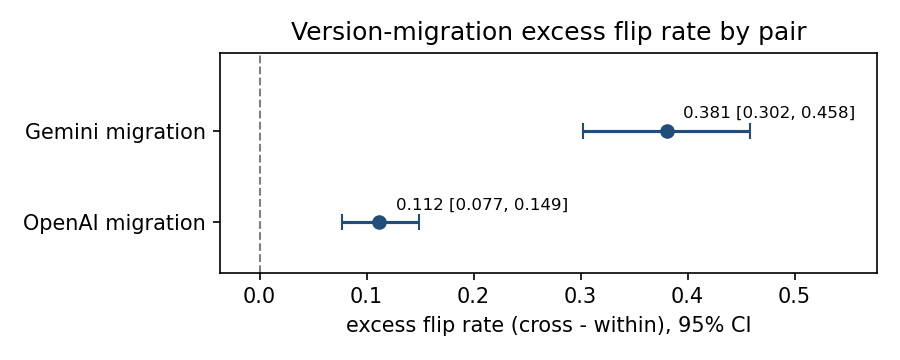
\includegraphics[width=\columnwidth]{fig1_excess_forest.png}
\caption{Excess flip rate (cross-version minus within-version noise floor) with 95\% CI for both migrations; both intervals exclude zero.}
\label{fig:forest}
\end{figure}

\subsection{The two shocks are structurally opposite}
The decomposition is where the two migrations diverge. OpenAI's gross flip is \emph{churn-dominated}: genuine per-company reconsideration (churn 0.122, 95\% CI [0.083, 0.161]) exceeds the marginal rating-mix shift (0.095), and cross-version agreement is moderate-to-substantial and consistent across estimators (Cohen 0.60, Scott 0.60, Gwet 0.70). Gemini's is \emph{marginal-dominated}: a wholesale re-rating (marginal 0.319) with only small---though still significant---per-name churn (0.070, 95\% CI [0.029, 0.120]) and lower agreement (Cohen 0.33). Operationally these are different failures: OpenAI re-judges \emph{which} companies are risky, Gemini re-rates the \emph{whole book}. A single flip-rate number would have hidden this distinction; the decomposition is what surfaces it.

\begin{figure}[t]
\centering
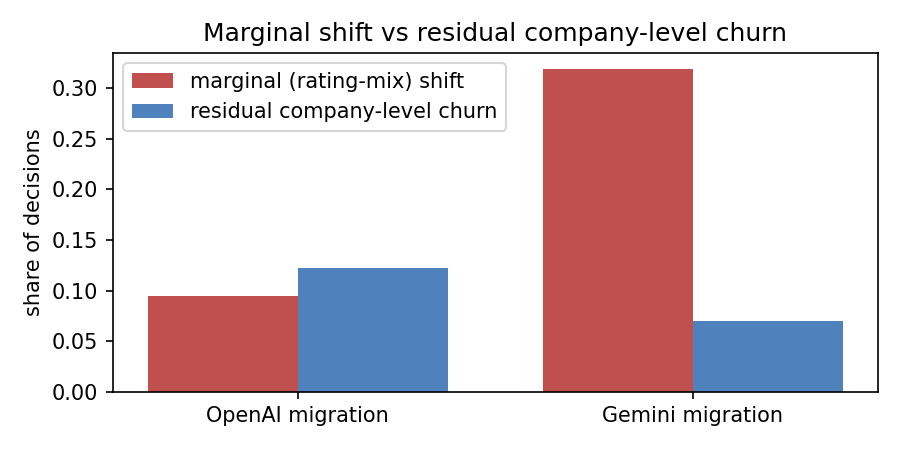
\includegraphics[width=\columnwidth]{fig2_prevalence.png}
\caption{Prevalence decomposition of the gross flip into a marginal (rating-mix) shift and genuine per-name churn. OpenAI is churn-dominated; Gemini is marginal-dominated.}
\label{fig:prev}
\end{figure}

\subsection{Directional drift: opposite directions}
Both migrations are strongly directional, but in opposite directions (Table~\ref{tab:mix}). OpenAI shifts assessments toward DISTRESS: the SAFE share falls from 0.30 to 0.21 while WATCH and DISTRESS rise, McNemar $p\approx6\times10^{-18}$. Gemini shifts sharply toward SAFE: the SAFE share \emph{rises} from 0.39 to 0.71 while DISTRESS nearly vanishes (0.086 to 0.012), McNemar $p\approx1.4\times10^{-59}$, with 0.201 tier turnover. One vendor's update made credit calls systematically harsher; the other's, systematically more lenient---on the identical task in the same period.

\begin{table}[t]
\centering
\caption{Credit-label mix before/after each migration. OpenAI shifts toward DISTRESS; Gemini shifts sharply toward SAFE.}
\label{tab:mix}
\small
\begin{tabular}{@{}lccc@{}}
\toprule
Version & SAFE & WATCH & DISTRESS \\
\midrule
OpenAI $v_{\mathrm{old}}$ & 0.304 & 0.588 & 0.108 \\
OpenAI $v_{\mathrm{new}}$ & 0.209 & 0.636 & 0.155 \\
Gemini $v_{\mathrm{old}}$ & 0.389 & 0.525 & 0.086 \\
Gemini $v_{\mathrm{new}}$ & 0.708 & 0.281 & 0.012 \\
\bottomrule
\end{tabular}
\end{table}

\begin{figure*}[t]
\centering
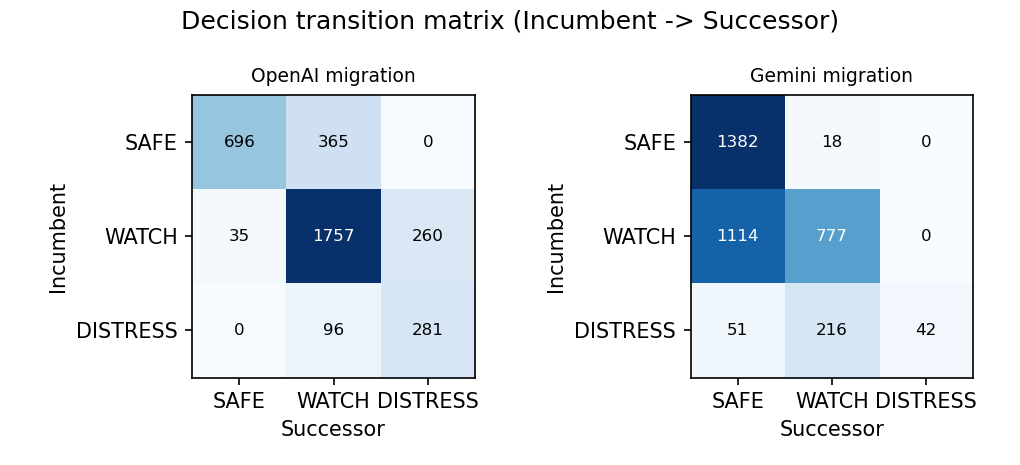
\includegraphics[width=0.72\textwidth]{fig3_transition.png}
\caption{Decision transition matrices ($v_{\mathrm{old}}\to v_{\mathrm{new}}$) for each migration. OpenAI's mass moves off the diagonal toward more-severe tiers; Gemini's moves sharply into SAFE.}
\label{fig:trans}
\end{figure*}

\subsection{Robustness of the agreement statistic}
The low cross-version agreement is not an artifact of one estimator's chance model. Cohen's $\kappa$, Scott's $\pi$, and Gwet's AC1 agree in ordering and rough magnitude for both pairs (Table~\ref{tab:main}); $\pi$ tracks $\kappa$ closely while AC1 is higher, as expected under skewed marginals, but the cross-vendor contrast (OpenAI substantially more concordant than Gemini) holds under all three.

\subsection{Instability dose-response}
Cross-version flips concentrate where the incumbent was already unstable across its own seeds: the flip rate in ``unstable'' cells exceeds that in ``stable'' cells by a contrast of $+0.330$ (OpenAI) and $+0.250$ (Gemini). Migration overturns decisions preferentially at genuine decision boundaries, consistent with a real reconsideration rather than uniform noise.

\begin{figure}[t]
\centering
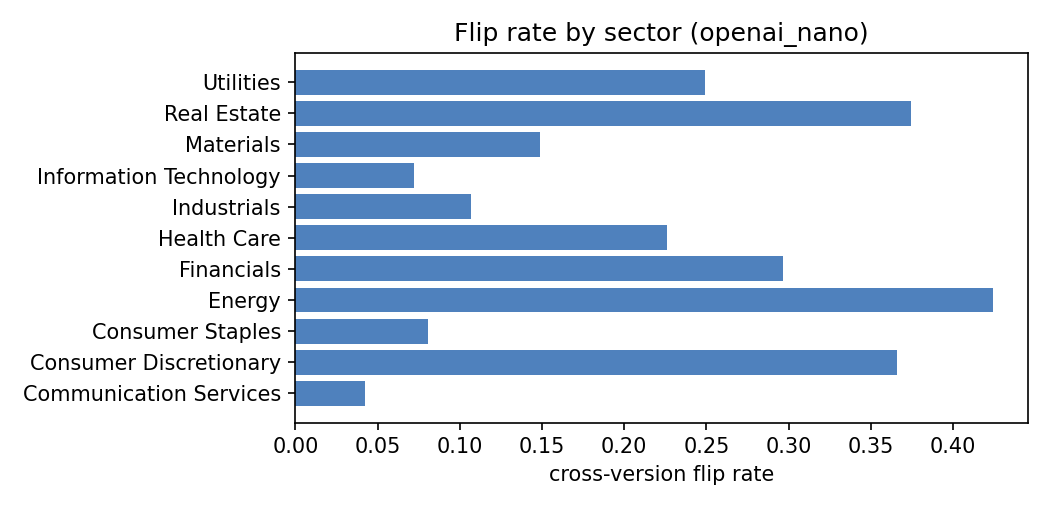
\includegraphics[width=\columnwidth]{fig4_sector.png}
\caption{Cross-version flip rate by GICS sector (openai\_nano); the shock is broad-based across sectors rather than driven by a single industry.}
\label{fig:sector}
\end{figure}

\subsection{Accuracy: an honest null in both cases}
\label{sec:acc}
Against the Altman ground truth (three-way chance 0.33), both versions of both pairs are competent, so the task is not one no model can perform: OpenAI 0.539$\to$0.564, Gemini 0.494$\to$0.425. But the flip-conditional accuracy change---does the migration improve the calls it overturns?---is $+0.124$ (95\% CI [$-0.164$, $+0.418$]) for OpenAI and $-0.179$ (95\% CI [$-0.380$, $+0.030$]) for Gemini; both span zero. Neither migration reliably improves correctness on the flipped cells. The shock is real, directional, and consequential, but not a skill improvement---forced credit-tier turnover with no compensating accuracy, and in Gemini's case a point estimate suggesting the more-lenient successor is if anything less aligned with distress.

\subsection{Temperature robustness}
The excess flip rate is re-estimated at $T\in\{0,0.7,1.0\}$ on a small $8\times3$ subgrid (24 cells; Table~\ref{tab:temp}). Point estimates are positive at all three temperatures for both pairs, so the effect is not a knife-edge of greedy decoding. We are deliberately careful about strength of claim here: because the subgrid is small the intervals are wide, and Gemini's $T{=}0$ lower bound touches zero, so the sweep establishes \emph{sign-stability}, not per-temperature significance; the load-bearing estimate remains the full-grid primary endpoint. Absolute levels rise mildly with $T$ (more sampling entropy), but the finding is the version contrast, which is temperature-stable.

\begin{table}[t]
\centering
\caption{Temperature-sensitivity robustness (excess flip rate with 95\% CI, $8\times3$ subgrid).}
\label{tab:temp}
\small
\begin{tabular}{@{}lcc@{}}
\toprule
$T$ & OpenAI & Gemini \\
\midrule
0.0 & 0.153 [.042,.278] & 0.222 [.000,.500] \\
0.7 & 0.167 [.056,.292] & 0.306 [.111,.500] \\
1.0 & 0.208 [.069,.361] & 0.389 [.167,.611] \\
\bottomrule
\end{tabular}
\end{table}

\section{Discussion}
\label{sec:disc}
Our central result gives quantitative teeth to a governance intuition: a routine vendor model update is not behavior-preserving for a fixed decision pipeline. On a task where the models are demonstrably competent, one update overturned about one in nine credit assessments and another more than one in three, both far above the sampling-noise floor, and both with astronomically significant directional drift. Because these updates are exogenous, forced by deprecation, and shared across every institution running the model, the shift is synchronized and cannot be diversified away within a single-vendor deployment.

The sharpest finding is that the two migrations are \emph{opposite}. Had we studied only one vendor we might have concluded ``updates make models harsher'' (OpenAI) or ``updates make models more lenient'' (Gemini); studying two shows neither generalizes. The direction, magnitude, and even the \emph{mechanism} (per-name reconsideration versus wholesale re-rating) are vendor-specific and, from the outside, unpredictable. For a risk manager this is worse than a uniform bias: a bias could be calibrated out, but an idiosyncratic, direction-unknown shock arriving on the vendor's schedule cannot be anticipated from experience with other vendors. The prevalence/churn decomposition is essential here: it is the instrument that distinguishes ``the book was re-rated'' from ``individual names were re-judged,'' and it is what shows the two shocks are structurally distinct rather than merely different in size.

\noindent\textbf{The ground-truth circularity objection.} Altman $Z''$ is a deterministic formula over the reported statements, so one might object that the task reduces to approximating a formula and that an LLM is superfluous. Three points defuse this. \emph{First}, the deployment the task represents is judgment-style screening: production credit-triage systems read heterogeneous, largely unstructured disclosures and render a holistic SAFE/WATCH/DISTRESS call; our prompt never mentions Altman, ratios, or any formula, so the model is asked for a judgment, not a computation, and the clean-statement input is a deliberately controlled harness chosen so that an objective label exists. \emph{Second}, $Z''$ is a validation instrument, not the deployment rationale---an external, reproducible yardstick for whether the model's judgments are non-random and whether migration changes correctness, exactly as a forward-return sign serves in related work; any objective label with these properties (realized default, an agency grade, a distress event) would serve, and we adopt $Z''$ because it is computable and reproducible. \emph{Third and decisively}, the primary result is \emph{label-free}: the excess flip rate, churn, agreement, and directional drift are computed entirely from the two versions' outputs against each other and never touch the ground truth, so the objection cannot reach the instability finding. Only the secondary accuracy linkage (Section~\ref{sec:acc}) uses $Z''$, and there our honest null makes no claim that the LLM is a good $Z''$ approximator.

\section{Governance: SR 11-7 and a Monitoring Control}
SR 11-7~\cite{sr117}---the foundational US model-risk framework from 2011 until it was superseded by the revised interagency guidance SR 26-2 in April 2026~\cite{sr2602}---organizes model risk around a lifecycle the institution controls: development, effective challenge and validation before use, ongoing monitoring, and change management, with explicit provisions for vendor and third-party models, whose use ``does not reduce the institution's responsibility for model risk management.'' Crucially, that guidance was written for a world in which the institution decides when a model changes: it contemplates the vendor model becoming \emph{unavailable} and requires contingency plans, but not the vendor \emph{silently replacing the model's behavior} beneath a live deployment, on the vendor's schedule, with forced deprecation. Version migration is the inverse of the anticipated risk---not loss of the model, but involuntary substitution of its behavior. Two features of the current landscape make this gap acute rather than academic: the 2026 revised guidance SR 26-2 explicitly places \emph{generative and agentic AI outside its scope}, deeming them too novel and rapidly evolving to govern~\cite{sr2602}, so the exact systems studied here fall in a supervisory gap; and where SR 26-2 does strengthen concentration and aggregate-exposure requirements, it does so at the \emph{enterprise} level (one institution's model portfolio), not across institutions. Our results make four provisions bite (Table~\ref{tab:gov}).

\noindent\textbf{Material change and accelerated review.} SR 11-7 requires review to be accelerated ``following material changes to the model.'' A migration is, by our measurement, a material change---excess flip 0.11--0.38 with directional drift at $p<10^{-17}$ in both pairs---yet the institution may never trigger the provision, because the change is vendor-initiated and the API surface (endpoint, model-family string) can be unchanged. The gap is \emph{detection}, not the requirement.

\noindent\textbf{Effective challenge before use.} Effective challenge presumes an independent, testable pre-change window; forced deprecation with limited notice compresses or removes it, so a successor can enter production without the critical, objective analysis the guidance requires.

\noindent\textbf{Inventory, change control, documentation.} A frozen model document is undermined by a moving model. Treating the exact snapshot string as a versioned artifact makes a vendor bump a tracked model change rather than an invisible configuration detail.

\noindent\textbf{Aggregate versus systemic risk---the missing provision.} SR 11-7 addresses aggregate model risk at the institution level, and SR 26-2 sharpens enterprise-level visibility into model concentrations and dependencies~\cite{sr2602}; but neither, to our reading of the primary texts, contemplates risk \emph{correlated across institutions} through a shared vendor update---the concern raised, at the market level, by supervisory work such as the ESRB Advisory Scientific Committee report on AI and systemic risk~\cite{esrb}. Our cross-vendor, synchronized result---two updates moving every deployment at once in vendor-specific, externally unpredictable directions---is exactly that systemic dimension at the decision level, and it sits outside the scope of current model-risk guidance (which, for generative AI, is empty by SR 26-2's own terms).

\noindent\textbf{A concrete control.} We propose a \emph{pre-migration parallel run} that satisfies these provisions at once. Before cutover, the institution runs the frozen pipeline on both incumbent and successor over a fixed, sector-stratified grid and computes the excess flip rate (net of the noise floor), the prevalence/churn decomposition, and the directional-drift test---yielding, in one procedure, the ongoing-monitoring signal that a material change occurred, the outcomes-analysis evidence (incumbent versus successor on identical inputs), and the effective-challenge artifact before use. A directionally-biased excess flip above a pre-registered materiality threshold gates cutover and triggers revalidation. Operationally: inventory the version string as a model version; contractually secure advance deprecation notice and the ability to pin the incumbent through a validation window; and retain the frozen incumbent as a challenger benchmark. We offer this as a practitioner-facing interpretation, not authoritative supervisory guidance; institutions should apply it through their own model-risk and compliance functions.

\begin{table*}[t]
\centering
\caption{Mapping vendor version migration to SR 11-7 provisions and the proposed control.}
\label{tab:gov}
\small
\begin{tabular}{@{}p{0.30\textwidth}p{0.37\textwidth}p{0.27\textwidth}@{}}
\toprule
SR 11-7 provision & How version migration breaks it & Proposed control \\
\midrule
Vendor/third-party responsibility \& contingency planning & Anticipates vendor-model \emph{loss}, not silent behavioral \emph{replacement} on the vendor's schedule & Inventory the exact version string; pin the incumbent through validation \\
Ongoing monitoring; accelerate review on material model change & The change is exogenous and silent (API surface unchanged), so it may never trigger the review it warrants & Pre-migration parallel run detects the change and quantifies its materiality \\
Effective challenge; validation before use & Forced deprecation with limited notice removes the pre-change testable window & Parallel-run gate provides challenge and validation evidence before cutover \\
Model inventory, change control, documentation & Frozen documentation undermined by a model that changes underneath it & Treat version-as-artifact; hash-pin the snapshot as the object of record \\
Aggregate (institution-level) model risk & Not contemplated as correlated \emph{across} institutions via a shared vendor update & Systemic gap; flagged for supervisory attention \\
\bottomrule
\end{tabular}
\end{table*}

\section{Threats to Validity}
\noindent\textbf{Seed non-determinism.} Reasoning models do not honor temperature deterministically; determinism relies on a best-effort vendor seed. The within-version flip rate quantifies the residual and is subtracted in the primary endpoint, so the headline is conservative; its large size relative to the floor (both pairs) confirms the effect is not sampling variance.

\noindent\textbf{Ground-truth choice.} Altman $Z''$ is an objective, reproducible label but a proxy for realized default; accuracy is reported as a secondary axis, and the primary instability result does not use it (Section~\ref{sec:disc}).

\noindent\textbf{Controlled harness, not a deployment simulation.} All results are for one credit-classification task with a single prompt template; magnitudes may differ on other tasks, though the mechanism---a vendor update changing a graded decision on identical inputs---is task-general. We acknowledge the setup is a controlled validation harness (clean reported statements as input, a formula-based label) rather than a full production simulation over heterogeneous, unstructured disclosures; this deliberately trades ecological realism for an objective, reproducible ground truth and clean isolation of the migration effect. An out-of-domain replication over unstructured inputs (e.g.\ filing red-flag detection) is the immediate next step.

\noindent\textbf{Provider and pair scope.} Two vendor migrations establish that the shock occurs and that its direction and mechanism differ across vendors, but two pairs cannot characterize the full distribution of migration behavior; a third pair (e.g. an xAI Grok migration) awaits a publicly available successor.

\noindent\textbf{Single-run collection.} Confirmatory data are collected once; provider-side drift within the collection window is not averaged out. Exact snapshot strings are pinned and the hash-frozen data is the object of record.

\section{Conclusion}
Two routine vendor updates each inflicted a large, significant shift in credit assessments on the identical task in the same period---one re-judging individual companies toward distress (OpenAI: one in nine assessments beyond the noise floor), the other re-rating the whole book toward safety (Gemini: more than one in three)---with genuine per-company reconsideration in the first case and a wholesale distributional shift in the second, and no accuracy gain in either, on a task where the models are demonstrably competent. Because the updates are exogenous, forced by deprecation, correlated across every institution running the model, and---as the two cases show---unpredictable in direction and mechanism across vendors, they constitute a synchronized, un-hedgeable decision shock that current model-risk governance does not see. We give the measurement, the prevalence/churn decomposition that both rules out a mere labeling artifact and exposes the cross-vendor difference, a temperature- and statistic-robustness suite, and a pre-migration parallel-run monitoring metric to detect the shock---all as a reproducible, pre-registered, build-gated artifact.

\section*{Data and Code Availability}
We release: (i) the immutable, read-only, SHA-256-stamped raw data (per-call model, seed, prompt hash, timestamp, tokens, cost, and raw response); (ii) the pre-registration, its cryptographic freeze receipt, and the amendments log; (iii) the deterministic, seeded analysis pipeline that regenerates every table byte-for-byte, with a build gate that rejects any manuscript number disagreeing with the frozen analysis; and (iv) the capture and monitoring harness (the pre-migration parallel-run metric). Artifacts are archived at [Zenodo DOI, to be minted on acceptance].

\section*{Acknowledgment}
The authors thank [reviewers/colleagues].

\begin{thebibliography}{99}
\small
\bibitem{muscle} J. Zhang \emph{et al.}, ``MUSCLE: A Model Update Strategy for Compatible LLM Evolution,'' arXiv:2407.09435, 2024. [Online]. Available: \url{https://arxiv.org/abs/2407.09435}
\bibitem{reliable} ``Beyond the Mean: Within-Model Reliable Change Detection for LLM Evaluation,'' arXiv:2604.27405, 2026. [Online]. Available: \url{https://arxiv.org/abs/2604.27405}
\bibitem{supply} ``Test Before You Deploy: Governing Updates in the LLM Supply Chain,'' arXiv:2604.27789, 2026. [Online]. Available: \url{https://arxiv.org/abs/2604.27789}
\bibitem{underspec} ``What Prompts Don't Say: Understanding Underspecification in LLM Tasks,'' arXiv:2505.13360, 2025.
\bibitem{kim} J. Kim \emph{et al.}, ``Correlated Errors in Large Language Models,'' arXiv:2506.07962, 2025. [Online]. Available: \url{https://arxiv.org/abs/2506.07962}
\bibitem{systemic} ``AI and Systemic Risk: Performative Prediction and Algorithmic Herding in Financial Markets,'' arXiv:2604.03272, 2026. [Online]. Available: \url{https://arxiv.org/abs/2604.03272}
\bibitem{homog} ``Representation Homogeneity and Systemic Instability in AI-Dominated Financial Markets,'' arXiv:2604.22818, 2026. [Online]. Available: \url{https://arxiv.org/abs/2604.22818}
\bibitem{esrb} S.\ Cecchetti, R.\ L.\ Lumsdaine, T.\ Peltonen, and A.\ S\'anchez Serrano, ``Artificial Intelligence and Systemic Risk,'' Reports of the ESRB Advisory Scientific Committee, No.~16, Dec.\ 2025.
\bibitem{sr117} Board of Governors of the Federal Reserve System and OCC, ``SR 11-7: Guidance on Model Risk Management,'' 2011.
\bibitem{sr2602} Board of Governors of the Federal Reserve System, OCC, and FDIC, ``SR 26-2: Revised Guidance on Model Risk Management,'' April 17, 2026 (supersedes SR 11-7); OCC Bulletin 2026-13.
\bibitem{mrm} ``Generative AI in Model Risk Management,'' Journal of Risk Model Validation, 2025.
\bibitem{gwet} K. L. Gwet, ``Computing inter-rater reliability and its variance in the presence of high agreement,'' British J.\ Math.\ Stat.\ Psychology, vol.~61, pp.~29--48, 2008.
\bibitem{altman} E. I. Altman, ``Financial Ratios, Discriminant Analysis and the Prediction of Corporate Bankruptcy,'' Journal of Finance, vol.~23, no.~4, pp.~589--609, 1968.
\bibitem{altman_em} E. I. Altman, ``An Emerging Market Credit Scoring System for Corporate Bonds,'' Emerging Markets Review, vol.~6, no.~4, pp.~311--323, 2005 (see also Altman, Hartzell, and Peck, 1995), which defines the $Z''$ model and its non-manufacturer / emerging-market cutoffs (2.6 / 1.1).
\end{thebibliography}

\vspace{1em}
\noindent\textbf{First A. Author} received the [B.S./M.S./Ph.D.] degree in [field] from [Institution], [City, Country]. [He/She] is currently [position] with [Department, Institution]. Research interests include large language models, model risk management, and reproducible empirical methods.

\vspace{0.4em}
\noindent\textbf{Second B. Author} received the [degree] in [field] from [Institution], [City, Country]. [He/She] is currently [position] with [Department, Institution]. Research interests include computational finance and machine-learning governance.

\end{document}
